% Main manuscript source. Compile from paper-draft/ with the section files.
\documentclass[11pt]{article}

\usepackage[margin=1in]{geometry}
\usepackage{amsmath,amssymb}
\usepackage{graphicx}
\usepackage{booktabs,array,tabularx,longtable}
\usepackage{xcolor}
\usepackage{pgfplots}
\pgfplotsset{compat=1.17}
\usetikzlibrary{positioning}
\usepgfplotslibrary{groupplots}
\usepgfplotslibrary{statistics}
\usepackage[hidelinks]{hyperref}
\urlstyle{same}
% Permit long reproducibility paths to wrap within identifiers.
\expandafter\def\expandafter\UrlBreaks\expandafter{\UrlBreaks
\do\a\do\b\do\c\do\d\do\e\do\f\do\g\do\h\do\i\do\j\do\k\do\l\do\m
\do\n\do\o\do\p\do\q\do\r\do\s\do\t\do\u\do\v\do\w\do\x\do\y\do\z}
\setlength{\emergencystretch}{3em}

\newcolumntype{Y}{>{\raggedright\arraybackslash}X}
\newcommand{\SO}{\mathrm{SO}}
\newcommand{\R}{\mathbb{R}}

\title{MorphMimic: Physics-Based Motion Imitation\\
for Diverse Human Body Shapes}
\author{[Author names and order]\\
\small [Department and institution]\\
\small [Corresponding author and email]}
\date{}

% Target: The Visual Computer. All reported measurements are retained.

\begin{document}
\maketitle
\begin{abstract}
Animating digital humans with different body proportions requires references
consistent with each body's geometry and a controller that tracks them in
physics. We present MorphMimic: a paired corpus that links 20,951 motion
identities to body-conditioned references and matching simulation assets for
128 body configurations, and one morphology-conditioned temporal controller
trained on 18,855 of these identities across all bodies. MorphMimic achieves
99.14\% tracking success on 1,048 held-out motions, with one selected trained
body per clip.
Replayed on 233 training-split clips across each of two panels of 128 unseen
bodies, success is 97.28\% inside the training coefficient range and 97.15\%
outside it, yet individual bodies succeed on as few as 3.0\% and 13.3\% of
clips, and a later checkpoint improves outside-panel success while regressing
individual bodies. In three-seed comparisons, attention variants reach higher
mean success and lower position error than a temporal multilayer perceptron
with less seed variability, while jerk differences stay within seed variation.
An offline audit of 19,200 references shows that refinement reduces
stance-foot sliding and below-floor body centres at the cost of higher
reference jerk. The evidence supports strong average tracking and transfer
within the evaluated domain; the causal contribution of explicit morphology
inputs and the mechanism of the severe failures remain open.
\end{abstract}

\noindent\textbf{Keywords:} Physics-based animation; Digital humans;
Motion imitation; Morphology-conditioned control; Temporal attention.


\section{Introduction}\label{sec:introduction}
Physics-based character animation should reproduce actions on digital humans
with different proportions and dynamics. A shared controller offers a way to
reuse a motion repertoire across those bodies, provided that references and
simulated assets remain consistent. Changing limb lengths, collision
geometry, and mass distribution changes both the spatial realization of a
motion and the actuation needed to track it. The learning problem therefore
has two coupled axes: variation in motion and variation in body. Good
tracking on new motions for a familiar body does not establish transfer to
a new body, and a high average over bodies can conceal severe failures.

Large motion resources, shape-conditioned reference generation, and scalable
imitation provide the building blocks~\cite{amass,humanml3d,humos,phc,protomotions}.
Body-conditioned control is established~\cite{won2019}. PHC and ASE learn from
motion collections but report results on a single body shape; PHC supports
body variation, although its quantitative evaluations use the mean SMPL
body~\cite{phc,ase} (Section~\ref{sec:external_comparison}). Our question is
how reliably one controller learns and transfers across a large corpus of
explicitly paired motions and bodies.

We approach it with a paired corpus in which every clip/body identity is
preserved from HUMOS generation through simulation and replay: 20,951 clip
identities and 128 body configurations, on which one shared temporal
slot/type-attention controller trains directly, using streamed motion
residency, on 18,855 clips. Evaluation separates motion exposure from body
exposure. The contributions are the paired corpus and workflow, the shared
controller configuration with streamed residency, exposure-separated
evaluation of trained and unseen bodies, and three-seed network comparisons
together with a reference-refinement audit.
We inherit the simulator integration, proximal policy optimization (PPO), and motion-tracking
infrastructure from ProtoMotions; we do not claim these or morphology
conditioning itself as new. HumanML3D captions are metadata, not policy
inputs: this is reference-conditioned imitation, not text-conditioned control.

The original checkpoint achieves 99.14\% success on 1,048 clip-disjoint test
clips, each paired with one selected trained body. On 233 training-split
clips across 128 unseen inside-range bodies and 128 unseen outside-range
bodies, success is 97.28\% and 97.15\%. Yet the worst bodies succeed on only
3.0\% and 13.3\% of those clips. These findings support the central claim:
\emph{one shared controller learns morphology-specific tracking with strong
average transfer to unseen shapes, but uneven robustness across individual
bodies}. The design evidence explains practical trade-offs; it does not yet
isolate the benefit of explicit morphology inputs or establish uniform
held-out-motion performance across all bodies.

The remainder of the paper is structured as follows.
Section~\ref{sec:related_work} reviews related work;
Section~\ref{sec:problem} defines the problem and system;
Section~\ref{sec:dataset} presents the corpus;
Section~\ref{sec:method} describes the proposed methodology;
Section~\ref{sec:experiments} specifies evaluation;
Section~\ref{sec:results} presents the results;
and Section~\ref{sec:discussion} discusses limitations and concludes.
The appendices provide reproducibility details,
training provenance, and additional unseen-body results; the complete per-body
tables are in the Supplementary Material.

\section{Related Work}\label{sec:related_work}

\paragraph{Physics-based motion imitation.}
DeepMimic showed that reference-guided reinforcement learning can produce
simulated character skills~\cite{deepmimic}, and Perpetual Humanoid Control
extended robust imitation to real-time simulated avatars~\cite{phc}. Both
motivate learning a feedback controller rather than replaying a kinematic
trajectory. PULSE learns a motion representation for humanoid control, OmniH2O,
ExBody2, and GMT study large-scale control on robot
platforms~\cite{pulse,omnih2o,exbody2,gmt}, and ASE learns reusable latent
skills rather than exact clip tracking~\cite{ase}; their published scores do not
measure our clip/body replay task. We build on ProtoMotions with Isaac Gym and
PPO~\cite{protomotions,isaacgym,ppo}.

\paragraph{Body variation and retargeting.}
Body-shape variation has been studied in physics-based control. Won and Lee
learned a parametric controller over character height, weight, and
proportions~\cite{won2019}, and ShapeVerse trains characters with varied SMPL
shape parameters to imitate walking and jogging~\cite{shapeverse}. Policies that
transfer across changes in agent \emph{topology}, such as limb count, use shared
modular sub-policies~\cite{smp2020}, a different axis from the continuous
variation studied here. Morphology conditioning is therefore established and
not claimed as new; we examine one controller over a large set of paired motions
and bodies, with shape identity maintained through generation, simulation, and
evaluation. Kinematic retargeting and dynamic tracking meet different
requirements. SMPL gives a common parameterized body~\cite{smpl}, SMPLSim builds
simulation-ready assets from it~\cite{smplsim}, and physics-based retargeting of
motion capture to realistic body shapes has been studied with spacetime
optimization~\cite{alborno2018}. A shared skeleton makes poses comparable but
does not make global positions or required actuation independent of shape, so
matching a reference to its simulation asset is part of the task definition.

\paragraph{Motion data and shape-conditioned generation.}
AMASS consolidates motion capture in a common body-model
representation~\cite{amass}, and HumanML3D associates processed segments with
natural-language descriptions~\cite{humanml3d}; we inherit these identities and
descriptions rather than claim new capture or shape-specific annotation. HUMOS
generates identity-conditioned motion with a cycle-consistent
formulation~\cite{humos}, and we use its pretrained model to obtain
shape-specific references, not as the controller. The sequences still need
conversion to the simulator's skeleton and a feasibility check there, and our
refinement is a deliberately limited kinematic post-process, not a new
generative model or trajectory optimizer. The controller uses standard
Transformer operations~\cite{attention}, and one ablation adapts the
zero-initialized adaptive layer normalization (adaLN) conditioning of
Diffusion Transformers~\cite{dit} to
actor-only morphology modulation; it tests a conditioning mechanism, not
diffusion-based action generation.

\paragraph{Comparison with related systems.}\label{sec:external_comparison}
Table~\ref{tab:capabilities} lists the reported tracking results of PHC and
ProtoMotions beside MorphMimic's. PHC, ASE, and ProtoMotions learn from motion
collections but report results on a single body shape. PHC evaluates on the mean
SMPL body, with optional shape-sampled training and no systematic unseen-body
panel~\cite{phc}; ASE reports task returns on one sword-and-shield humanoid
rather than tracking success~\cite{ase}; and ProtoMotions documents configurable
characters and a fall-based success rate~\cite{protomotions}. Won and Lee
establish parametric body control, with experiments that differ from our
clip-by-body panels~\cite{won2019}; as neither they nor ASE report a comparable
tracking success, both are left out of the table. PHC's success criterion matches ours (joint
error above 0.5\,m at any point), but motions, clip lengths, bodies, and reference sources (captured versus generated) differ,
so the rows are not a ranking; no external system has been rerun under our
protocol, our quantitative design comparison is internal, and no performance
advantage is claimed. MorphMimic's distinction is the combination of many
motions and many body shapes under one controller, with references and assets
paired per body and systematic inside- and outside-range replay.

\begin{table}[t]
\centering\small\setlength{\tabcolsep}{4pt}
\caption{Reported tracking results of PHC, ProtoMotions, and MorphMimic.}\label{tab:capabilities}
{\footnotesize
\begin{tabularx}{\linewidth}{@{}p{0.165\linewidth}YrYYrr@{}}
\toprule
System & Training set & Motions & Evaluated on & Bodies & \shortstack[r]{Succ.\\(\%)} & \shortstack[r]{$E_{\text{g-mpjpe}}$\\(mm)} \\
\midrule
PHC~\cite{phc} & AMASS & 11,313 & AMASS-Train & 1 (mean SMPL) & 98.9 & 37.5 \\
 & & & AMASS-Test (140) & 1 (mean SMPL) & 96.4 & 47.4 \\
ProtoMotions~3~\cite{protomotions} & AMASS & 40+\,h & AMASS (docs) & 1 per character & $\approx$99\textsuperscript{a} & --- \\
\midrule
MorphMimic & HUMOS references from AMASS & 18,855 & Held-out test (1,048) & 128 (one per clip) & 99.14 & 67.6 \\
 & & & Inside range (233) & 128 unseen & 97.28 & 98.8 \\
 & & & Outside range (233) & 128 unseen & 97.15 & 95.1 \\
\bottomrule
\end{tabularx}}

\smallskip
\begin{minipage}{\linewidth}\footnotesize
Succ.: joint error $\le0.5$\,m at every frame (PHC's criterion; Eq.~\eqref{eq:success}).
$E_{\text{g-mpjpe}}$: global mean per-joint position error, for MorphMimic over all
clips including failures. \textsuperscript{a}Fall-only criterion. ``---'': not reported.
Both PHC and MorphMimic exclude object-interaction sequences.
\end{minipage}
\end{table}

\paragraph{Inherited functions and study additions.}
ProtoMotions provides the simulation abstraction, PPO training, and
motion-library and imitation infrastructure, HUMOS supplies the pretrained
generator, and SMPL and SMPLSim supply the body parameterization and assets. We
add the paired corpus assembly and identity checks, the reference processing and
fidelity audit, the evaluated slot/type controller configuration, streamed clip
residency, and exposure-separated evaluation. These are system and empirical
contributions built on existing methods, not claims to invent attention, PPO,
body models, or motion imitation.

\section{Overview}\label{sec:problem}
A body configuration $b=(g,\boldsymbol{\beta})$ specifies a SMPL template
and shape coefficients. For source clip $c$, HUMOS supplies a shape-specific
reference $\hat{s}_{c,b}(t)$ and SMPLSim supplies the matching asset. Changing
$b$ changes geometry, reference positions, mass/inertia, and mass-scaled
actuation even though topology is shared, so the task is to track these paired
references with one policy rather than impose identical world-space paths on
all bodies.

MorphMimic learns $\pi_\theta(a_t\mid o_t,b)$ from the present state, history,
future reference targets, and body information, with the same parameters
serving every body. Clips can change on reset while each environment retains
its asset, and evaluation preserves reference/body identity. The flat-ground
task has no external objects or partners, and captions are metadata, not
controller input.

Figure~\ref{fig:data_pipeline} summarizes the system. Matching body parameters
link generated references and simulation assets (Section~\ref{sec:dataset});
the policy is defined in Section~\ref{sec:method} and trained on the resulting
pairs with streamed motion residency (Section~\ref{sec:training}); and fixed
pairs with known motion and body exposure are replayed for evaluation
(Section~\ref{sec:results}).

\begin{figure}[t]
\centering
\fbox{\begin{minipage}{0.94\linewidth}
\small
\begin{tabularx}{\linewidth}{@{}p{0.12\linewidth}Y@{}}
\textbf{Motion} &
AMASS $\longrightarrow$ HumanML3D preprocessing and clip extraction
$\longrightarrow$ HUMOS conditioned on $(g,\boldsymbol{\beta})$
$\longrightarrow$ MotionLib conversion and reference refinement
$\longrightarrow$ per-clip motion variants. \\[0.7em]
\textbf{Body} &
SMPL with the same $(g,\boldsymbol{\beta})$
$\longrightarrow$ SMPLSim
$\longrightarrow$ matching skeleton, collision geometry, mass/inertia,
and MuJoCo XML (MJCF) asset identity. \\[0.7em]
\textbf{Text} &
HumanML3D source descriptions
$\longrightarrow$ clip-ID lookup associated with the generated variants
(metadata only; not a policy input).
\end{tabularx}

\smallskip
The body assets are used for motion conversion, shape-specific forward
kinematics, ground-clearance correction, and simulation. Refined reference
motion and matching simulated state feed one shared policy.
\end{minipage}}
\caption{Paired reference and simulation-asset construction.}\label{fig:data_pipeline}
\end{figure}

\section{Paired Motion and Body Corpus}\label{sec:dataset}

We construct a derived corpus in which a source clip identity connects a motion
description, 128 generated motion variants, and their matching simulation
assets. A \emph{clip} denotes a source segment, including a mirrored segment
when present; a \emph{variant} denotes that clip on one body configuration.
Figure~\ref{fig:data_pipeline} shows the construction paths.

\subsection{Source motion and body configurations}\label{sec:source_data}

\paragraph{Motion.}
We use the AMASS-derived motion portion of HumanML3D~\cite{amass,humanml3d},
drawn from the 18 source collections listed in
Appendix~\ref{app:preprocessing}. Source SMPL+H sequences are processed at
20\,Hz, with clip extraction, temporal cropping, mirroring, and
treadmill/skating cleanup following the HumanML3D/HUMOS pipeline, so
HumanML3D identities are preserved. The pipeline produced 22,459 candidate
clip identities, counting original and mirrored clips; a text-based filter
removed 1,508 that appear to require external objects or environmental
support, leaving 20,951 identities for flat-ground imitation. The filter is a
task-scope heuristic and does not prove that every retained reference is
support-free or dynamically feasible. HumanML3D descriptions stay associated
with the variants of their source clip as metadata; their semantic fidelity is
not audited (Appendix~\ref{app:captions}), and they supply keyword-based motion
classes only for the exploratory analysis in Section~\ref{sec:physics}.

\paragraph{Bodies.}
A body configuration is $b=(g,\boldsymbol{\beta})$, where $g$ identifies the
female or male SMPL variant and $\boldsymbol{\beta}\in\R^{10}$ contains shape
coefficients. We sample
\begin{equation}
    \beta_{ij}\sim\mathcal{U}(-3,3),\qquad
    i=1,\ldots,64,\quad j=1,\ldots,10,
    \label{eq:shape_sampling}
\end{equation}
and cross the 64 vectors with the two variants, giving 128 body configurations
rather than 128 independent coefficient vectors. Uniform sampling is a
controlled source of variation, not a representative sample of human
populations.

\paragraph{Reference and asset generation.}
For each clip, the pretrained HUMOS model~\cite{humos} receives the processed
pose and root features and the target body parameters, and returns a
shape-conditioned reference (root-relative 6D rotations with translation). In
parallel, SMPL bodies~\cite{smpl} with identical parameters are converted to
MJCF assets with SMPLSim~\cite{smplsim}, using mass estimation and hand and
foot simplifications. Each asset has 24 rigid bodies and 69 actuated joint
coordinates, with its own collision proxies, joint ranges, and estimated masses
and inertias. These are simulation-model estimates, not measurements of human
participants.

\subsection{Reference conversion and refinement}\label{sec:refinement}

Generated sequences are converted to ProtoMotions' Z-up convention and
resampled from 20 to 30\,Hz. Forward kinematics (FK) uses the matching asset
rather than a single neutral skeleton, and the packaged representation stores
global body positions and rotations, local rotations, joint positions,
velocities, and contact labels. Refinement is applied independently to each
variant in five steps; default settings are in
Table~\ref{tab:refinement_parameters}.

\emph{Contacts.} Ankle and toe contacts are validated, or detected from foot
position and velocity when labels are unusable; short gaps are closed and very
short runs removed. These label candidate stance intervals and are not measured
forces. \emph{Rotation filtering.} Joint rotations are filtered with
sign-continuous quaternions, normalization, and a bounded geodesic correction;
contact transitions divide the sequence into segments so that filtering does
not average across a change of stance. \emph{Root correction.} A conservative
least-squares root translation, anchored at each contact's median foot
position, reduces horizontal stance sliding. It is temporally regularized and
capped, so it does not guarantee exact foot locking and does not solve for new
joint angles. \emph{Ground clearance.} With floor height zero and margin
$\epsilon_z$, the lift required at frame $t$ is
\begin{equation}
    \ell_t^{\mathrm{req}}
      = \max\!\left(0,\epsilon_z-\min_{x\in\mathcal{C}_b(t)}x_z\right),
    \label{eq:clearance}
\end{equation}
where $\mathcal{C}_b(t)$ is the collision geometry of body $b$, and a smoothed
lift envelope stays above this requirement. This prevents penetration of the
checked geometry in the reference; it does not establish balanced support,
realistic impacts, or freedom from self-collision. \emph{Reconstruction.} FK
and velocities are recomputed from the corrected root and rotations within
each motion.

The objective is modest: reduce measurable kinematic artifacts while preserving
the generated motion. Section~\ref{sec:refinement_results} reports artifact and
fidelity measures; improved kinematics alone does not demonstrate improved
policy learning or dynamic feasibility.

\subsection{Scale and splits}\label{sec:splits}

Each per-clip file stores the 128 variants with frame counts, sampling rates,
and the clip and asset identities needed to recover body parameters, so the
training system can stream clip files without downloading the complete corpus.
Splits are by clip identity: all variants of a clip, and original/mirrored
partners, share a partition (Table~\ref{tab:dataset_counts}), and variants are
generated combinations rather than independent captures. The split is
versioned with seed 42 and roughly 90/5/5 proportions; the 150 development
clips used for design comparisons and the reference audit are reserved within
the training split (Appendix~\ref{app:provenance}), and the test manifest is
never loaded by the training workflow. The splits test held-out clip identities
on the trained body set. They have not been shown to be disjoint by subject or
capture recording, which limits claims about broader motion generalization.

\begin{table}[t]
\centering
\caption{Corpus and split sizes.}\label{tab:dataset_counts}
\begin{tabular}{lrr}
\toprule
Partition & Clip identities & Motion variants \\
\midrule
Training & 18,855 & 2,413,440 \\
Validation & 1,048 & 134,144 \\
Test & 1,048 & 134,144 \\
\midrule
Total & 20,951 & 2,681,728 \\
\bottomrule
\end{tabular}
\end{table}

\section{Policy}\label{sec:method}
MorphMimic's controller is the policy $\pi_\theta(a_t\mid o_t,b)$ of
Section~\ref{sec:dataset}: it maps the present state, history, future reference
targets, and morphology to joint targets. This section defines its states and
actions, network, reward, and training.

\paragraph{State.}
Experiments use the \texttt{smpl\_mor} assets in Isaac Gym through
ProtoMotions~\cite{isaacgym,protomotions}, with simulation at 60\,Hz, two
substeps, and control decimation two, giving a 30\,Hz policy rate. The
observation combines the present state, history, future reference targets, a
historical action, and explicit morphology information. Let $B=24$ denote the
number of simulated bodies. The present state contains root height above
ground, root-relative body positions excluding the root, 6D body rotations, and
linear and angular velocities. Positions and velocities use a heading-aligned
frame and rotations remove the root heading, which removes dependence on
arbitrary global heading and horizontal origin while retaining height and body
configuration. We add seven historical states at control-step offsets
$\{1,2,3,4,8,16,32\}$, covering about 1.07\,s and each in its own root/heading
frame, and four future reference slots at $\{1,2,4,8\}$, covering about
0.27\,s. Future slots contain target positions relative to the current root,
heading-aligned target rotations, position differences from the current body
state, relative rotations $\smash{R_{t,j}^{-1}\hat{R}_{t+k,j}}$ (expressed with
respect to the current body rotation), and heading-aligned linear and angular
velocity differences. The history exposes recent changes and the future targets
a short anticipation window; contact flags, an explicit phase scalar, text, and
estimated physical feature vectors are not part of the observation.
Table~\ref{tab:observations} summarizes the inputs of actor and critic, with
dimensions per slot, positions in metres, linear velocities in m/s, angular
velocities in rad/s, and dimensionless 6D rotations.

\begin{table}[t]
\centering
\small
\caption{Observation inputs supplied to both actor and critic.}\label{tab:observations}
\begin{tabularx}{\linewidth}{@{}lrlY@{}}
\toprule
Input & Dimension & Slots & Representation and path \\
\midrule
Current state & $15B-2=358$ & 1 &
Height; $3(B-1)$ positions; $6B$ rotations; $3B$ linear and $3B$ angular
velocities. Current-state encoder. \\
History & $358$ & 7 &
Same state representation at the seven past offsets. Shared history encoder. \\
Future reference & $24B=576$ & 4 &
Target and relative poses ($18B$), plus velocity differences ($6B$).
Shared future encoder. \\
Historical action & $D=69$ & 1 &
A raw previous policy-action vector, before the tanh and joint-target mapping.
Bypasses attention. \\
Morphology & $11$ & 1 &
$[g,\beta_1,\ldots,\beta_{10}]$ from the assigned asset.
Bypasses attention. \\
\bottomrule
\end{tabularx}
\end{table}

\paragraph{Action.}
The policy outputs a raw action $a_t\in\R^D$ with $D=69$, mapped to joint
targets by
\begin{equation}
    q_t^{\mathrm{target}}
      = q^{\mathrm{offset}}
        + q^{\mathrm{scale}}\odot\tanh(a_t),
    \label{eq:action_mapping}
\end{equation}
with offsets and scales derived from the configured joint ranges. The targets
drive the simulator's built-in position proportional--derivative (PD)
controller; the action is not a residual added to the reference pose. PD
stiffness, damping, and effort limits are scaled per joint by the mass of the
associated rigid body relative to that body in the reference asset (base values
in Appendix~\ref{app:control}). This body-level mass scaling is not a single
scale based on total character mass, and it does not guarantee dynamically
equivalent actuation across geometrically different bodies.

\paragraph{Network.}
MorphMimic uses temporal slot/type attention. Three observation encoders, one
for the current state, one shared across history slots, and one shared across
future slots, are multilayer perceptrons (MLPs) with two 256-unit hidden layers,
rectified linear unit (ReLU) activations, and a 256-dimensional token output, and their inputs use running mean/standard-deviation
normalization with a magnitude clamp of five. The resulting 12 tokens (one
current, seven historical, four future) enter a Transformer as
\begin{equation}
    z_i = E_{\tau(i)}(x_i)
        + e_i^{\mathrm{slot}} + e_{\tau(i)}^{\mathrm{type}},
    \qquad i=0,\ldots,11,
    \label{eq:token_embedding}
\end{equation}
where $\tau(i)$ identifies the current, history, or future source: slot
embeddings distinguish the configured temporal offsets, and type embeddings the
observation sources. The Transformer has two layers, four attention heads, token
width 256, and feed-forward width 1,024~\cite{attention}, and its current-state
token supplies the pooled output after the configured output projection and
activation. Figure~\ref{fig:network} traces the encoded observations through
attention and the separate actor and critic heads, which share input categories
but not parameters.

\begin{figure}[t]
\centering
\fbox{\begin{minipage}{0.94\linewidth}
\small
\begin{tabularx}{\linewidth}{@{}YcY@{}}
Current state: $1\times358$ & $\longrightarrow$ &
Current encoder: $1\times256$ token \\
Past states: $7\times358$ & $\longrightarrow$ &
History encoder: $7\times256$ tokens \\
Future targets: $4\times576$ & $\longrightarrow$ &
Future encoder: $4\times256$ tokens
\end{tabularx}
\begin{center}
$\downarrow$\\
12 tokens + learned temporal-slot and source-type embeddings\\
$\downarrow$\\
2 Transformer layers, 4 heads, width 256\\
$\downarrow$\\
Pool current token: $h_t\in\R^{256}$\\
$\downarrow$\\
Concatenate $[h_t,\ a^{\mathrm{hist}}_t,\ g,\boldsymbol{\beta}]$
and normalize
\end{center}
\begin{tabularx}{\linewidth}{@{}YY@{}}
\textbf{Actor:} six 2,896-unit layers
$\longrightarrow$ 69 action means
$\longrightarrow$ tanh/range scaling
$\longrightarrow$ PD targets. &
\textbf{Critic:} four 1,024-unit layers
$\longrightarrow$ scalar state value.
\end{tabularx}
\smallskip
The entire encoder/attention pathway is instantiated separately for actor
and critic; the drawing summarizes the common design, not shared weights.
Morphology and action bypass attention into each head. Text is absent.
\end{minipage}}
\caption{Temporal slot/type controller and separate actor/critic heads.}\label{fig:network}
\end{figure}

The final head input concatenates the 256-dimensional attention output, the
historical raw action, and the 11-dimensional morphology vector; this
336-dimensional input also uses running normalization and clamp five. Betas are
not manually divided by three, embedded as a separate attention token, or used
for adaLN modulation in the selected model. Actor and critic have separate token
encoders, attention modules, slot/type embeddings, and MLP heads, with six
hidden layers of width 2,896 for the actor and four of width 1,024 for the
critic, all with ReLU activations; they output a Gaussian action mean and a
scalar value, respectively. PPO samples actions with fixed diagonal log standard
deviation $-2.9$, and evaluation uses the mean action.

\paragraph{Reward.}
The training reward combines global body tracking and root-height tracking. For
corresponding simulated and reference body positions $p_j,\hat{p}_j$, rotations
$R_j,\hat{R}_j$, and velocities $v_j,\hat{v}_j$ and $\omega_j,\hat{\omega}_j$,
define
\begin{align}
    e_p &= \frac{1}{3B}\sum_{j=1}^{B}\|p_j-\hat{p}_j\|_2^2,
    \\
    e_R &= \frac{1}{B}\sum_{j=1}^{B}
                  d_{\SO(3)}(R_j,\hat{R}_j)^2, \\
    e_v &= \frac{1}{3B}\sum_{j=1}^{B}\|v_j-\hat{v}_j\|_2^2,
    \\
    e_\omega &= \frac{1}{3B}\sum_{j=1}^{B}
                     \|\omega_j-\hat{\omega}_j\|_2^2, \\
    e_h &= (h-\hat{h})^2,
\end{align}
where $d_{\SO(3)}$ is the geodesic rotation angle in radians and the
coordinate-wise means in the position and velocity errors match the implemented
reductions. The reward is
\begin{equation}
\begin{split}
    r_t ={}& 0.5\exp(-25e_p) + 0.3\exp(-5e_R)
             + 0.1\exp(-0.5e_v)\\
           &+0.2\exp(-0.1e_\omega) + 0.2\exp(-100e_h),
\end{split}\label{eq:reward}
\end{equation}
with weights that are not normalized to sum to one. There is no explicit
effort, action-smoothness, or contact-matching reward in this experiment, and no
source-dependent switch between canonical and HUMOS reward functions.

\paragraph{Optimization.}
MorphMimic is trained directly across all bodies on refined HUMOS references,
with no neutral pretraining stage, using PPO~\cite{ppo}. References are sampled
only from variants matching the environment's asset.
Reference-state initialization starts at frame zero with probability 0.2 and
otherwise at a random valid reference time. Training episodes last at most
1,000 control steps and terminate on falls (a 0.15\,m height setting, with
permitted foot-contact bodies), while tracking-error termination is disabled, so
this rule is distinct from the evaluation failure threshold of
Section~\ref{sec:metrics}. PPO uses 32-step rollouts, discount 0.99, generalized
advantage estimation (GAE) parameter 0.95, policy-ratio clipping 0.2, normalized
advantages, and separate Adam optimizers with learning rates $2\times10^{-5}$ for
the actor and $10^{-4}$ for the critic. Other settings and the actual run budgets
are in Appendix~\ref{app:training}.

\paragraph{Streamed motion sampling.}
The full-scale experiment streams per-clip files through
\texttt{GlobalClipPool}. The training manifest is deterministically partitioned
across GPU ranks, and each rank keeps a bounded resident pool containing all 128
variants of its selected clips, with environment-level motion sampling
respecting the assigned morphology. The pool is rebuilt every 256 epochs: most
slots are selected by priority, combining estimated clip difficulty and an
exploration bonus, and a fraction 0.2 is reserved for uniform random selection
to maintain rehearsal outside the highest-priority set. This is a training
curriculum, not uniform sampling of the complete corpus. Validation membership
is fixed independently of pool rebuilding and does not update sampling weights,
so resident-pool and validation metrics measure different populations. Sampling
constants and the pool size actually used are in
Appendices~\ref{app:reproducibility} and~\ref{app:history}.

\section{Training}\label{sec:training}
MorphMimic is trained directly across all bodies on refined HUMOS references,
with no neutral pretraining stage, using PPO~\cite{ppo}.

\paragraph{Optimization.}
References are sampled only from variants matching the environment's asset.
Reference-state initialization starts at frame zero with probability 0.2 and
otherwise at a random valid reference time. Training episodes last at most
1,000 control steps and terminate on falls (a 0.15\,m height setting, with
permitted foot-contact bodies), while tracking-error termination is disabled, so
this rule is distinct from the evaluation failure threshold of
Section~\ref{sec:metrics}. PPO uses 32-step rollouts, discount 0.99, GAE
parameter 0.95, policy-ratio clipping 0.2, normalized advantages, and separate
Adam optimizers with learning rates $2\times10^{-5}$ for the actor and
$10^{-4}$ for the critic. Other settings and the actual run budgets are in
Table~\ref{tab:training_parameters} (Appendix~\ref{app:reproducibility}).

\paragraph{Streamed motion sampling.}
The full-scale experiment streams per-clip files through
\texttt{GlobalClipPool}. The training manifest is deterministically partitioned
across GPU ranks, and each rank keeps a bounded resident pool containing all 128
variants of its selected clips, with environment-level motion sampling
respecting the assigned morphology. The pool is rebuilt every 256 epochs: most
slots are selected by priority, combining estimated clip difficulty and an
exploration bonus, and a fraction 0.2 is reserved for uniform random selection
to maintain rehearsal outside the highest-priority set. This is a training
curriculum, not uniform sampling of the complete corpus. Validation membership
is fixed independently of pool rebuilding and does not update sampling weights,
so resident-pool and validation metrics measure different populations. Sampling
constants and the pool size actually used are in
Appendices~\ref{app:reproducibility} and~\ref{app:history}.

\section{Evaluation}\label{sec:results}
We evaluate MorphMimic on held-out motions, on trained bodies, and on unseen
bodies, and use per-body failures to delimit the claims. Each reference is
rolled out only in an environment using its exact asset identity, so a
reference is never assigned to a different body. Evaluation uses the mean action
and reference initialization, disables training termination, and records errors
over the valid reference horizon, capped at 600 control steps (20\,s at 30\,Hz),
so success refers to the evaluated horizon, not necessarily the whole source
clip. Held-out evaluations select one body variant per clip with a deterministic
hash of the clip identity (Appendix~\ref{app:reproducibility}), so the clip list
is fixed while the body panel rotates across scheduled evaluations. Validation
was monitored repeatedly and is not an untouched test set, whereas the
clip-disjoint test manifest stays outside training and model selection and is
evaluated once.

Design comparisons run on a development corpus of 150 clips and all 128 body
configurations (19,200 variants), reserved within the training split; it is not
a held-out generalization benchmark. Because compute was limited, architecture
and reference-processing choices are investigated on this subset with a fixed
simulation budget, whereas the full-scale run trains on the 18,855 training
clips (Table~\ref{tab:dataset_counts}). An exploratory analysis of cross-body
control demand on the same clips was inconclusive and is reported in
Appendix~\ref{app:physics}. Table~\ref{tab:evidence_populations}
lists all populations; held-out identity is clip-grouped, not a demonstrated
subject or recording split.

\begin{table}[!htb]
\centering\small
\caption{Evaluation populations; each unseen panel has 128 bodies.}
\label{tab:evidence_populations}
\begin{tabularx}{\linewidth}{@{}lYYr@{}}
\toprule
Evaluation & Motion exposure & Body exposure & Pairs \\
\midrule
Validation / test & Held-out clips & Trained; one per clip & 1,048 each \\
Development replay & 150 training clips & All 128 trained & 19,200 \\
Unseen inside / outside & 233 training clips & All 128 unseen per panel & 29,824 each \\
Unseen diagnostic subset & 23 val/test clips; seen by full-data & Same unseen panels & 2,944 each \\
Trained-body control & 150 training clips & All 128 trained & 19,200 \\
Design comparison & Development clips & Trained bodies & Three refined seeds \\
\bottomrule
\end{tabularx}
\end{table}

\paragraph{Metrics.}\label{sec:metrics}
For each evaluated clip/shape pair $i$, the per-frame mean body position error is
\begin{equation}
    d_{i,t} = \frac{1}{B}\sum_{j=1}^{B}
                 \|p_{i,t,j}-\hat{p}_{i,t,j}\|_2 ,
\end{equation}
and the configured success indicator is
\begin{equation}
    S_i = \mathbf{1}\!\left[
             \max_{t<T_i}d_{i,t}\leq 0.5\ \mathrm{m}
          \right],
    \label{eq:success}
\end{equation}
where $T_i$ is the evaluated horizon. This threshold is deliberately distinct
from the smoother training reward, and passing it does not imply fine-grained
pose accuracy or biomechanical realism. We also report success at the stricter
thresholds 0.3, 0.2, and 0.1\,m, time-averaged mean
body-position error (the global mean per-joint position error $E_{\text{g-mpjpe}}$ of Table~\ref{tab:capabilities}), mean global body-rotation geodesic error (not a local
joint-angle error), the time average of the largest body-position error within
each frame (the logged \emph{mean maximum-joint error}), and the windowed
normalized jerk of Appendix~\ref{app:smoothness}, whose high-jerk statistic is
the percentage of windows in which any body exceeds 6,500. Errors are averaged
over valid frames per motion and then over motions, including failed rollouts;
offline comparisons aggregate saved per-motion records over unique clip/shape
pairs.

\paragraph{Held-out motions on selected trained bodies.}\label{sec:test_results}
The epoch-28,170 MorphMimic checkpoint was re-evaluated offline with a
standalone evaluator, once on the validation split and once on the clip-disjoint
test split, with one selected body per clip (shape panel index 110;
Table~\ref{tab:test_results}). All 1,048
clips of each split last about 6.6\,s (198 evaluated frames), so none reaches the
600-step cap. The test manifest is loaded only by this evaluator, which first
verifies its hash, clip count, and disjointness from train and validation; the
test split was evaluated once and not used to select the checkpoint.

\begin{table}[t]
\centering
\small
\caption{Offline evaluation of MorphMimic (epoch 28,170) on validation and test splits.}\label{tab:test_results}
\begin{tabular}{lrr}
\toprule
Metric & Validation & Test \\
\midrule
Success at 0.5\,m (\%) $\uparrow$ & 98.47 & 99.14 \\
Nominal 95\% Wilson interval, 0.5\,m (\%) & [97.53, 99.06] & [98.38, 99.55] \\
Success at 0.3\,m (\%) $\uparrow$ & 95.52 & 96.28 \\
Success at 0.2\,m (\%) $\uparrow$ & 84.83 & 85.97 \\
Success at 0.1\,m (\%) $\uparrow$ & 37.88 & 38.55 \\
Failure rate at 0.5\,m (\%) $\downarrow$ & 1.53 & 0.86 \\
Mean body-position error (m) $\downarrow$ & 0.0699 & 0.0676 \\
Mean global body-rotation error (rad) $\downarrow$ & 0.1738 & 0.1723 \\
Mean maximum-joint position error (m) $\downarrow$ & 0.1419 & 0.1393 \\
Normalized jerk $\downarrow$ & 1,154.3 & 1,050.9 \\
High-jerk windows (\%) $\downarrow$ & 27.46 & 25.33 \\
Worst single clip, gt err max (m) & 3.79 & 1.67 \\
\bottomrule
\end{tabular}
\end{table}

Validation and test scores are similar (1,032 and 1,039 of 1,048 successes at
0.5\,m), and no significance claim is made from their difference. The 0.5\,m
threshold is permissive, so the table also reports stricter thresholds and
continuous errors: test success falls to 96.28\% at 0.3\,m, 85.97\% at 0.2\,m,
and 38.55\% at 0.1\,m. Tight thresholds partly measure the references rather
than the controller, because HUMOS generates them kinematically and they are
not dynamically validated; the refinement audit below
finds residual contact artifacts even after refinement. The Wilson
intervals~\cite{wilson1927} are nominal: they condition on the checkpoint and
selected body panel and ignore dependence between related recordings or
mirrored clips, training variability, and uncertainty across body selections.

\paragraph{Coverage of trained bodies.}
Replaying 150 training clips on all 128 trained bodies (19,200 pairs) reaches
99.29\% success with the same checkpoint (Table~\ref{tab:unseen_v2}), which
establishes broad tracking on that subset. All-body consistency on held-out
motions remains unmeasured: it would need a held-out-motion panel crossed with
all 128 bodies. Figure~\ref{fig:trained_multibody_demo} shows one motion tracked
on the 128 trained bodies; it illustrates execution and does not quantify
tracking, contact quality, or transfer.

\paragraph{Residual failures.}\label{sec:failures}
Nine test and 16 validation pairs fail the threshold. Their captions suggest
ground transitions (six test, five validation failures) and whole-body
rotations (two test, four validation), and also mention turning, side-stepping,
an abrupt stop, and a hand-held sparring stick absent from simulation. These
describe the failed sample rather than mechanical causes or class-specific
failure rates; diagnosis would need synchronized rollouts and first-crossing
traces, including successful variants of the same clips.

\paragraph{Unseen-body panels.}
Each panel contains 64 new coefficient vectors instantiated on male and female
SMPL templates. Inside vectors lie in $[-3,3]^{10}$; outside vectors have
$\|\beta\|_\infty\in(3,5]$, with 16 vectors (32 bodies) in each of four
half-unit tiers. Inside denotes membership of the training coefficient box, not
of the convex hull of trained bodies. Both panels use matching HUMOS references
and assets, frame-zero offsets, and full reference refinement; the build report
records zero penetration under its refinement diagnostic but does not certify
dynamic feasibility. Replay uses mean actions, reference initialization, 32
environments per asset, and at most 210 control steps (7\,s), with success as in
Eq.~\eqref{eq:success}. The 233 training-split identities isolate the body axis,
while the other 23 validation/test identities remain separate; the trained-body
control uses a different 150-clip panel and refinement run, so only
within-dataset checkpoint deltas are paired comparisons.

\paragraph{High average transfer inside and outside the training range.}
Crossing the 233 training-split clips with all 128 bodies in each panel gives
29,824 pairs per panel, and Table~\ref{tab:unseen_v2} includes every body and
every failed pair. MorphMimic's original checkpoint reaches 97.28\%
inside-range and 97.15\% outside-range success. The trained-body control reaches 99.29\%, but uses
different clips and a different refinement run, so the gap of roughly two
percentage points (pp) is descriptive, not a matched estimate of the effect of
changing bodies. Deltas are paired within each dataset, 95\% confidence
intervals (CI) resample clips
with the body panel fixed, and the rerun repeats the original checkpoint, not its
training.

\begin{table}[!htb]
\centering\small
\caption{Unseen-body success of the original and later checkpoints, with the
trained-body control.}\label{tab:unseen_v2}
\begin{tabularx}{\linewidth}{@{}YrrrY@{}}
\toprule
Panel & \shortstack{Refined\\(\%)} & \shortstack{Full-data\\(\%)} & \shortstack{Rerun $\Delta$\\(pp)} & Candidate $\Delta$ [95\% CI] (pp) \\
\midrule
Inside unseen & 97.28 & 96.91 & $-0.02$ & $-0.37$ [$-0.57$, $-0.18$] \\
Outside unseen & 97.15 & 97.57 & $+0.04$ & $+0.42$ [$+0.22$, $+0.61$] \\
Trained control & 99.29 & 99.12 & $+0.02$ & $-0.17$ [$-0.37$, $-0.03$] \\
\bottomrule
\end{tabularx}
\end{table}

\paragraph{Failures concentrate in individual bodies.}
High averages coexist with severe body-specific failures. Inside body
\texttt{male\_669a0fb3} succeeds on 3.0\% of clips and outside body
\texttt{male\_1c099619} on 13.3\%; another inside body, \texttt{male\_ec3bb7f8},
reaches only 19.3\% despite an in-range mass of 42.7\,kg and height of 1.41\,m.
Figure~\ref{fig:unseen_v2_shapes} shows all 128 bodies of each panel, sorted
independently by original-checkpoint success on the same 233 known clips (the
ranking does not pair inside and outside bodies), and Online Resource 1 reports
every body. Lying outside the training coefficient box does not explain
these failures: success does not decline monotonically across the four outside
coefficient tiers (99.03, 97.76, 95.33, and 96.47\%). Bodies outside the trained
height range perform well on average (97.91\% outside; 96.42\% inside), while
the tallest in-range bin is weaker (90.53\% outside; 88.75\% inside). The eight
heaviest outside bodies, above 144.4\,kg, average 79.02\%, but small overlapping
property groups and paired male/female templates are not independent samples of
physical-property space, so coefficient extremity, mass, and height give no
simple ordering of transfer difficulty (tier and mass tables in
Appendix~\ref{app:unseen_tables}). All failed rows have zero recorded
termination flags; because flags depend on the replay configuration rather than
an independent fall detector, we treat these as threshold failures pending
synchronized rollouts and contact and root-height traces.

\begin{figure}[t]
\centering
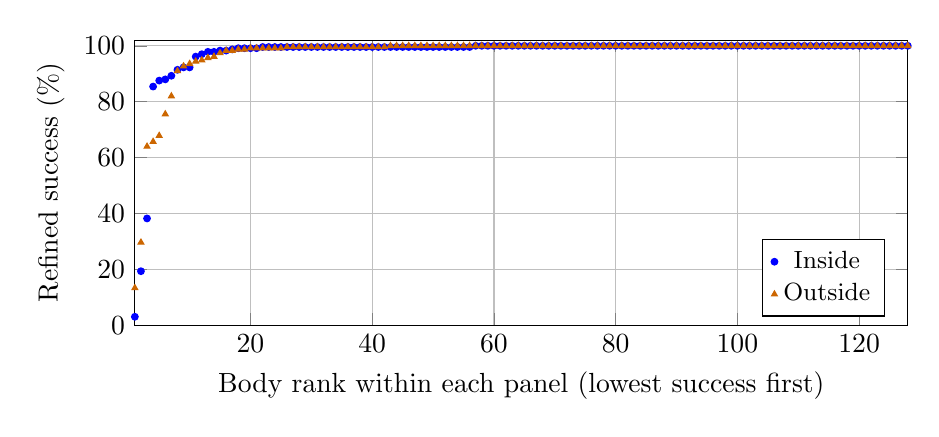
\begin{tikzpicture}
\begin{axis}[width=0.94\linewidth,height=5.2cm,
xlabel={Body rank within each panel (lowest success first)},
ylabel={Refined success (\%)},xmin=1,xmax=128,ymin=0,ymax=102,
legend pos=south east,legend style={font=\small},grid=major]

\addplot[only marks,mark=*,mark size=1.2pt,blue] coordinates {
(1,3.00) (2,19.31) (3,38.20) (4,85.41) (5,87.55) (6,87.98) (7,89.27) (8,91.42) (9,92.27) (10,92.27) (11,96.14) (12,97.00) (13,97.85) (14,97.85) (15,98.28) (16,98.28) (17,98.71) (18,99.14) (19,99.14) (20,99.14) (21,99.14) (22,99.57) (23,99.57) (24,99.57) (25,99.57) (26,99.57) (27,99.57) (28,99.57) (29,99.57) (30,99.57) (31,99.57) (32,99.57) (33,99.57) (34,99.57) (35,99.57) (36,99.57) (37,99.57) (38,99.57) (39,99.57) (40,99.57) (41,99.57) (42,99.57) (43,99.57) (44,99.57) (45,99.57) (46,99.57) (47,99.57) (48,99.57) (49,99.57) (50,99.57) (51,99.57) (52,99.57) (53,99.57) (54,99.57) (55,99.57) (56,99.57) (57,100.00) (58,100.00) (59,100.00) (60,100.00) (61,100.00) (62,100.00) (63,100.00) (64,100.00) (65,100.00) (66,100.00) (67,100.00) (68,100.00) (69,100.00) (70,100.00) (71,100.00) (72,100.00) (73,100.00) (74,100.00) (75,100.00) (76,100.00) (77,100.00) (78,100.00) (79,100.00) (80,100.00) (81,100.00) (82,100.00) (83,100.00) (84,100.00) (85,100.00) (86,100.00) (87,100.00) (88,100.00) (89,100.00) (90,100.00) (91,100.00) (92,100.00) (93,100.00) (94,100.00) (95,100.00) (96,100.00) (97,100.00) (98,100.00) (99,100.00) (100,100.00) (101,100.00) (102,100.00) (103,100.00) (104,100.00) (105,100.00) (106,100.00) (107,100.00) (108,100.00) (109,100.00) (110,100.00) (111,100.00) (112,100.00) (113,100.00) (114,100.00) (115,100.00) (116,100.00) (117,100.00) (118,100.00) (119,100.00) (120,100.00) (121,100.00) (122,100.00) (123,100.00) (124,100.00) (125,100.00) (126,100.00) (127,100.00) (128,100.00)
};\addlegendentry{Inside}
\addplot[only marks,mark=triangle*,mark size=1.2pt,orange!80!black] coordinates {
(1,13.30) (2,29.61) (3,63.95) (4,65.67) (5,67.81) (6,75.54) (7,81.97) (8,90.99) (9,92.70) (10,93.56) (11,94.42) (12,94.85) (13,95.71) (14,96.14) (15,97.42) (16,98.28) (17,98.28) (18,98.71) (19,98.71) (20,99.14) (21,99.14) (22,99.14) (23,99.14) (24,99.14) (25,99.14) (26,99.57) (27,99.57) (28,99.57) (29,99.57) (30,99.57) (31,99.57) (32,99.57) (33,99.57) (34,99.57) (35,99.57) (36,99.57) (37,99.57) (38,99.57) (39,99.57) (40,99.57) (41,99.57) (42,99.57) (43,100.00) (44,100.00) (45,100.00) (46,100.00) (47,100.00) (48,100.00) (49,100.00) (50,100.00) (51,100.00) (52,100.00) (53,100.00) (54,100.00) (55,100.00) (56,100.00) (57,100.00) (58,100.00) (59,100.00) (60,100.00) (61,100.00) (62,100.00) (63,100.00) (64,100.00) (65,100.00) (66,100.00) (67,100.00) (68,100.00) (69,100.00) (70,100.00) (71,100.00) (72,100.00) (73,100.00) (74,100.00) (75,100.00) (76,100.00) (77,100.00) (78,100.00) (79,100.00) (80,100.00) (81,100.00) (82,100.00) (83,100.00) (84,100.00) (85,100.00) (86,100.00) (87,100.00) (88,100.00) (89,100.00) (90,100.00) (91,100.00) (92,100.00) (93,100.00) (94,100.00) (95,100.00) (96,100.00) (97,100.00) (98,100.00) (99,100.00) (100,100.00) (101,100.00) (102,100.00) (103,100.00) (104,100.00) (105,100.00) (106,100.00) (107,100.00) (108,100.00) (109,100.00) (110,100.00) (111,100.00) (112,100.00) (113,100.00) (114,100.00) (115,100.00) (116,100.00) (117,100.00) (118,100.00) (119,100.00) (120,100.00) (121,100.00) (122,100.00) (123,100.00) (124,100.00) (125,100.00) (126,100.00) (127,100.00) (128,100.00)
};\addlegendentry{Outside}
\end{axis}\end{tikzpicture}
\caption{Unseen-body success, sorted within each panel.}\label{fig:unseen_v2_shapes}
\end{figure}

\paragraph{Checkpoint sensitivity.}
The later full-data checkpoint (epoch 34,000) was trained on all original motion
splits and differs from the original (epoch 28,170, distinct from the epoch-28,159
monitoring snapshot of Appendix~\ref{app:history}) by $-0.37$ pp inside and
$+0.42$ pp outside (Table~\ref{tab:unseen_v2}). Paired 95\% bootstrap intervals
resample clips with the body panel fixed, not training seeds or unseen bodies,
and a change counts as beyond noise only if its interval excludes zero and its
magnitude exceeds the identical-checkpoint rerun delta; both changes qualify,
but duration and motion coverage changed together, so they cannot be attributed
to either, and without a checkpoint ladder ordinary checkpoint variation remains
unmeasured. Identical-checkpoint reruns agree on 99.33\% of inside and 98.68\%
of outside pair labels (99.96\% in the control), yet individual pairs can change
by metres in peak error, so small pooled changes coexist with local instability.
The outside gain is concentrated in the ten bodies beyond the trained mass range
($+7.68$ pp, 95\% CI [$+6.39$, $+9.01$]) and the outermost coefficient tier
($+1.39$ pp [$+1.07$, $+1.72$]), while mean position error rises by 2.4, 5.0, and
3.1\,mm in the outside, inside, and control panels, so threshold success and
continuous tracking move differently. Three inside and six outside bodies regress
by more than 2 pp with intervals excluding zero, by up to 36.5 pp (per-body
intervals are exploratory and unadjusted for multiple testing), and five outside
bodies improve by more than 2 pp, including \texttt{male\_1c099619} (13.3\% to
71.2\%) (Appendix~\ref{app:unseen_tables}); neither improved extremes nor a
higher outside average justify calling the later checkpoint uniformly better. On
the 23-clip diagnostic subset, which the later checkpoint trained on, inside
success is 97.08\% versus 96.50\% and outside 96.81\% versus 96.91\% for the
original and later checkpoints; these values are excluded from the headline.
Severe failures remain unresolved: per-asset reference feasibility and
synchronized contact, root-height, and actuation traces have not been audited, so
reference, controller, and asset mechanisms cannot be distinguished.

\paragraph{Design comparisons.}\label{sec:design}
We compare four architectures: A, temporal MLP; B, temporal attention; C,
attention with slot/type embeddings, the architecture of MorphMimic; and D, C
with actor-only adaLN-Zero. All retain morphology inputs in actor and critic.
Refined-reference runs use three seeds (0, 1, 2) and a matched 6,000-epoch
budget on the development subset (Table~\ref{tab:architecture_seeds}), and each
run contributes one summary, the mean
of its last eight evaluations (epochs 4,600--6,000); means and sample standard
deviations are computed across the three run summaries, and within-run
evaluations are not replicates. Seed-1/2 values were checked against local
TensorBoard records, whereas the original logs of the seed-0 values were not
independently available. The full-scale MorphMimic model predates these reruns, which
reassess its design rather than establish prospective selection. Cases E--H
repeat A--D with unrefined references and one seed each
(Appendix~\ref{app:history}).

\begin{table}[t]
\centering\small
\caption{Three-seed refined-reference comparison, mean $\pm$ standard deviation across seeds.}\label{tab:architecture_seeds}
\begin{tabularx}{\linewidth}{@{}Yrrrrr@{}}
\toprule
Architecture & Success (\%) & Pos. (m) & Rot. (rad) & Jerk & Params (M) \\
\midrule
A: temporal MLP & $95.14\pm2.07$ & 0.118 & 0.216 & $2{,}110\pm643$ & 65.9 \\
B: temporal attention & $97.56\pm0.34$ & 0.090 & 0.218 & $2{,}783\pm887$ & 51.2 \\
C: slot/type attention & $97.89\pm0.22$ & 0.090 & 0.219 & $2{,}413\pm762$ & 51.2 \\
D: C + adaLN-Zero & $97.17\pm0.08$ & 0.083 & 0.211 & $2{,}659\pm674$ & 52.1 \\
\bottomrule
\end{tabularx}
\end{table}

Position and rotation errors are across-seed means, and parameters are actor
and critic totals. Attention variants reach 97.2--97.9\% mean success against
95.1\% for the temporal MLP, with lower position error (0.083--0.090 versus
0.118\,m) and much smaller seed variability (standard deviation 0.08--0.34
versus 2.07 points), although the MLP has the most parameters, roughly
26--29\% more than the attention variants. Among the attention variants, C has
the highest mean success and D the lowest position and rotation errors. A has
the lowest mean jerk, but jerk differences between architectures are
comparable to the seed-to-seed standard deviations (643--887), so the apparent
factor-of-two jerk advantage in seed 0 is not a consistent architecture
effect. Three seeds do not establish statistical superiority, and MorphMimic
uses C as a practical compromise.

\paragraph{Reference refinement.}\label{sec:refinement_results}
A paired offline audit of all 19,200 development references (150 clips
$\times$ 128 bodies; no simulation) compares artifact and fidelity measures
before and after refinement (Table~\ref{tab:refine_audit}). Artifact rows give
the corpus mean before and after and the fraction of motions that improve;
fidelity rows give the corpus mean refined-versus-unrefined difference.
Refinement lowers stance-foot speed during detected contact from 0.055 to
0.038\,m/s, with 96\% of references improving, and below-floor frames from
39.6\% to 3.3\% (only 45\% of references improve on the latter because many
were already grounded). Measured motion features are largely preserved: the mean
per-body rotation change is $0.12^\circ$, root horizontal displacement is
0.008\,m, and the cross-shape variance of knee-flexion range is retained at a
ratio of 0.94. The cost is higher reference jerk (the raw mean third difference
of body positions, not the windowed evaluator score), from 45.2 to
60.7\,m/s$^3$, with 79\% of references worsening; temporal root and clearance
corrections are a candidate explanation, but their contribution to policy
smoothness is not isolated. Refined and unrefined policies (cases A--D versus
E--H) track different targets, so their comparison describes different tasks
and does not establish a causal benefit of refinement, which would need a
common-reference checkpoint comparison.

\begin{table}[!htb]
\centering
\small
\caption{Reference-refinement audit over 19,200 development references.}\label{tab:refine_audit}
\begin{tabularx}{\linewidth}{@{}Yrrr@{}}
\toprule
& Unref.\ mean & Refined mean & Motions improved \\
\midrule
Stance-foot speed (m/s) $\downarrow$ & 0.055 & 0.038 & 96\% \\
Frames below floor (\%) $\downarrow$ & 39.6 & 3.3 & 45\% \\
Frames within 2\,cm of floor (\%) $\downarrow$ & 49.8 & 33.6 & --- \\
Position jerk (m/s$^3$) & 45.2 & 60.7 & 21\% \\
\midrule
Per-body rotation change (deg) & \multicolumn{3}{c}{0.12} \\
Root horizontal displacement (m) & \multicolumn{3}{c}{0.008} \\
Cross-shape var., knee-flexion range (ratio r/u) & \multicolumn{3}{c}{0.94} \\
\bottomrule
\end{tabularx}
\end{table}

\paragraph{Scope of the morphology-conditioning evidence.}
Every architecture receives morphology inputs in actor and critic. The adaLN-Zero
variant changes how the actor uses them but does not test their removal, and
body-dependent state and reference targets also expose morphology. Successful
transfer therefore establishes a capability of the whole system, not that
explicit coefficients cause it. Attributing it to those inputs needs a matched
training run without them, with the same references, body panel, budget, and
seeds; inference-time masking or shuffling would introduce distribution shift
and cannot replace that comparison.

\section{Discussion and Limitations}\label{sec:discussion}
MorphMimic combines paired morphology-specific references and assets with one
temporal controller and an evaluation that separates motion exposure from body
exposure. Trained across 128 bodies, it achieves 99.14\% success on held-out
motions with one selected trained body per clip and executes development clips
across all trained bodies. It transfers to unseen bodies at 97.28\% inside and
97.15\% outside the training coefficient range, but individual bodies can fail
on most clips, and a later checkpoint introduces both recoveries and
regressions. Temporal attention improves tracking accuracy and seed stability
over a temporal MLP without a consistent smoothness difference, and the
reference audit shows reduced contact artifacts at the cost of higher reference
jerk. These comparisons support practical architecture and reference-processing
choices, but not a causal explanation of transfer.

\paragraph{Implications for character animation.}
Body-specific references and one shared feedback controller support reuse across
the tested digital-human configurations. The reference audit and the
simulated-motion results are complementary: reference cleaning does not
establish lower sliding or penetration in controller outputs, which remain
unassessed, and high threshold success is tracking capability, not a complete
assessment of visual realism.

\paragraph{Average transfer and individual robustness.}
Similar inside and outside averages do not make body extrapolation uniformly
reliable. Success is non-monotonic across coefficient tiers, and poor tracking
occurs both beyond and within the training mass and height ranges; these
associations describe the tested assets and do not identify failure causes. The
later checkpoint recovers some bodies and harms others, so threshold success
alone would overstate its improvement.

\paragraph{Coverage and inference.}
The unseen-body headline uses known motion identities to isolate body transfer,
the 1,048-clip test uses one trained body per clip, and a fixed held-out-motion
panel crossed with all 128 trained bodies remains missing. Original and mirrored
variants stay together, but the splits are not shown to be subject- or
recording-disjoint. Clip-bootstrap intervals hold the body panel fixed and do not
quantify uncertainty over shape space, and one full-scale run with one candidate
checkpoint does not measure training-seed or ordinary checkpoint variation.

\paragraph{Mechanism and design.}
Attributing transfer to explicit morphology inputs needs the matched run
described in Section~\ref{sec:design}; the architecture comparison keeps those
inputs in every model and has unequal capacities, with the temporal MLP the
largest. Refinement reduces contact artifacts with small pose changes but raises
target jerk, and policies evaluated against different targets do not isolate its
learning benefit. The exploratory physical analysis
(Section~\ref{sec:physics}) remains descriptive.

\paragraph{Failure diagnosis and scope.}
Failures are error-threshold failures with zero termination flags, which alone
do not prove the absence of falls. Synchronized rollouts, contact and root
trajectories, and per-asset feasibility audits are needed before assigning a
mechanism; extreme HUMOS references have been refined but lack such validation.
Estimated masses, collision proxies, and mass-scaled gains are modeling choices,
and tracking success and jerk do not certify biomechanical realism. The short,
reference-initialized flat-ground protocol excludes objects, partners,
long-horizon recovery, skeletal-topology changes, and real robots. The corpus is
derived, so clip/body variants are not independent captures, and caption
alignment is not audited. A matched external tracker would strengthen
comparative conclusions, but the published capability comparison alone cannot
establish a performance advantage.

\paragraph{Summary and outlook.}
The evidence supports strong average shared tracking and transfer within this
protocol. All-body held-out-motion coverage, matched conditioning and external
controls, and dynamic diagnosis of severe failures remain necessary for
stronger claims about robustness and mechanism.

\section*{Acknowledgements}
For the purpose of open access, the authors have applied a Creative Commons
Attribution (CC BY) licence to any Author Accepted Manuscript version arising
from this submission.

\section*{Statements and Declarations}
% Author metadata and declarations remain provisional at the authors' request.
\paragraph{Funding}
The authors did not receive support from any organization for the submitted work.

\paragraph{Competing interests}
The authors have no relevant financial or non-financial interests to disclose.

\paragraph{Author contributions}
Longzhen Han conceived the study, developed the methodology and software,
generated the data, and ran most of the experiments and analysis. Beck
Farrington-Wheeler contributed substantially to the training
experiments and the non-software work, with further contributions from Sajjad
Hussain. Almas Baimagambetov and Nikolaos Polatidis supervised the work. All authors approved the final manuscript.

\paragraph{Data and code availability}
The motion corpus derives from AMASS and HumanML3D and remains subject to
the source datasets' access and licensing conditions; it is not distributed.
The research code repository is \url{https://github.com/hansen1416/morph_mimic}
(version \texttt{v1.0}), and demonstrations are available at
\url{https://hansen1416.github.io/morph_mimic/}. The repository contains the
experiment files, the data-preparation, evaluation and analysis tools, the
simulation models of the 128 trained and the $2\times128$ unseen-panel bodies
(derived from SMPL and released with attribution), their shape coefficients, and
the clip-identifier lists and split record. The epoch-28,170 MorphMimic checkpoint
evaluated in this paper (SHA-256 in Appendix~\ref{app:reproducibility}) is available at
\url{https://huggingface.co/YugoAmaryl/morph-mimic} under a non-commercial licence;
the epoch-34,000 checkpoint is not released. Reproducing the evaluations requires
the motion corpus, or references regenerated with the released pipeline.
Evaluation summaries and per-body results used in this manuscript are in
Online Resource 1; the per-motion validation and test records are retained with
the research records.

\paragraph{AI assistance in manuscript preparation}
An AI assistant was used to help restructure and draft manuscript text and
check consistency with the recorded sources. Reported experimental
measurements come from existing research records; this assistance did not
produce new training or rollout results.
% Submission package: authors to supply final affiliations, correspondence,
% author biographies and portrait photographs separately.


\appendix
\section{Reproducibility Details}\label{app:reproducibility}

\subsection{Source preparation and refinement settings}\label{app:preprocessing}

The AMASS source collections used by the preparation pipeline are ACCAD,
BioMotionLab\_NTroje, BMLhandball, BMLmovi, CMU, DFaust\_67, EKUT,
Eyes\_Japan\_Dataset, HumanEva, KIT, MPI\_HDM05, MPI\_Limits, MPI\_mosh,
SFU, SSM\_synced, TCD\_handMocap, TotalCapture, and Transitions\_mocap.
Source preparation operates at 20\,Hz; the final motion libraries use
30\,Hz. Joint ordering and quaternion conventions must follow the matching
asset and MotionLib conversion rather than be inferred from source array
positions. Body coefficients are sampled with NumPy's random number generator
using seed 46, and bodies are identified by stable beta keys rather than
content hashes. SMPLSim assets use mass estimation and hand and foot
simplifications (\texttt{real\_weight}, \texttt{replace\_feet},
\texttt{remove\_toe}, \texttt{freeze\_hand}).

\begin{table}[htbp]
\centering
\small
\caption{Default settings of the current reference-refinement procedure.
Frame counts refer to the 30\,Hz MotionLib representation. These are
kinematic-processing settings, not physical constraints learned by the policy.}\label{tab:refinement_parameters}
\begin{tabularx}{\linewidth}{@{}lY@{}}
\toprule
Operation & Setting \\
\midrule
Contact candidates & Left/right ankle and toe bodies \\
Contact detection thresholds & Speed 0.15\,m/s; height 0.10\,m \\
Contact cleanup & Close gaps up to 2 frames; remove runs shorter than 3 frames \\
Rotation filter & Savitzky--Golay, 9-frame window, polynomial order 3 \\
Rotation blend / bound & Strength 0.5; maximum geodesic correction $8^\circ$ \\
Contact-transition guard & Separate segments; 2-frame transition taper \\
Root XY correction & Median stance anchors; least-squares common translation \\
Root correction regularization & 21-frame smoothing window; 0.10\,m displacement cap \\
Ground clearance & 0.005\,m collision-geometry margin; 5-frame lift smoothing \\
Final reconstruction & Per-asset FK and per-motion velocity recomputation \\
\bottomrule
\end{tabularx}
\end{table}

\subsection{Caption provenance}\label{app:captions}

HumanML3D descriptions are available through a separate clip-ID lookup and the
annotation metadata used by HUMOS. A description is associated with the
variants of its source clip; it is not a new annotation for each generated body.
A coarse check against a single-caption-per-clip lookup finds a caption for all
20,951 clip identities, but semantic fidelity is not established: of the 9,579
mirrored identities, 22\% carry a caption byte-identical to their un-mirrored
source and 40\% contain an explicit left/right or clockwise term that mirroring
inverts, so removing a mirror prefix does not establish a correct caption.
Segment timing and multi-annotation coverage against the full HumanML3D
annotation set are not audited, and the keyword-based motion classes used in
Section~\ref{sec:physics} have not been manually validated. The retained and
excluded ID lists provide the audit trail for the object-support filter.

\subsection{Training configuration}\label{app:training}

Table~\ref{tab:training_parameters} records the shared optimization settings and
the environment and batch sizes actually used; run-specific resolved
configurations take precedence over older launch examples. The full-scale frame
count is a recorded stopping snapshot, not a budget matched to the development
runs. Clip priority combines estimated difficulty, updated from training-pool
evaluations with an exponential moving average of rate 0.1 and a floor of 0.05,
and an exploration coefficient of 1.0; the pool is rebuilt every 256 epochs and
a fraction 0.2 of slots is reserved for uniform selection.

\begin{table}[t]
\centering
\small
\caption{Training configuration; environment and minibatch counts are per GPU.}\label{tab:training_parameters}
\begin{tabularx}{\linewidth}{@{}lYY@{}}
\toprule
Setting & Corrected 150-clip runs & Full-scale MorphMimic run \\
\midrule
Parallel GPUs per policy & 1 & 6 \\
Environments per GPU & 4,096 & 2,048 \\
PPO minibatch size per GPU & 16,384 & 8,192 \\
Rollout length & 32 control steps & 32 control steps \\
Mini-epochs per update & 1 & 1 \\
Actor / critic learning rates &
$2\times10^{-5}$ / $10^{-4}$ & $2\times10^{-5}$ / $10^{-4}$ \\
Discount / GAE / ratio clip & 0.99 / 0.95 / 0.2 & 0.99 / 0.95 / 0.2 \\
Gradient norm clip & 50 & 50 \\
Evaluation cadence & 200 epochs & 256 epochs \\
Training seed & 0--2 (refined A--D); 0 (unrefined E--H) & 0 (saved run configuration) \\
Reference residency & All 150 clips & 256, later 128 clips per GPU \\
Training frames & 786,432,000 per run (6,000 epochs) & Approximately $11.07\times10^9$ recorded \\
Status of reported evidence & Completed, Table~\ref{tab:architecture_seeds} & Epoch-28,170 checkpoint, Table~\ref{tab:test_results} \\
\bottomrule
\end{tabularx}
\end{table}

\subsection{PD gains and limits}\label{app:control}

Table~\ref{tab:pd_parameters} gives the base values configured for the
SMPL morphology robot. For joint $d$ belonging to rigid body $j$, the
simulator applies the multiplier
\begin{equation}
    \rho_{b,j} = \frac{m_{b,j}}{m_{\mathrm{ref},j}}
\end{equation}
to stiffness, damping, and effort limit. The velocity limit is not mass-scaled.
All relevant asset masses, joint ranges, collision settings, and the reference
asset must accompany a reproducible physical interpretation.

\begin{table}[htbp]
\centering
\small
\caption{Base PD and actuation values before per-body mass scaling.
Stiffness and damping use the simulator's rotational PD units
(Nm/rad and Nm\,s/rad); effort limits are in Nm and velocity limits in rad/s.}\label{tab:pd_parameters}
\begin{tabular}{lrrrr}
\toprule
Joint family & Stiffness & Damping & Effort limit & Velocity limit \\
\midrule
Hip, knee, ankle & 800 & 80 & 500 & 100 \\
Toe & 500 & 50 & 500 & 100 \\
Torso, spine, chest & 1,000 & 100 & 500 & 100 \\
Neck, head, thorax, shoulder, elbow & 500 & 50 & 500 & 100 \\
Wrist, hand & 300 & 30 & 500 & 100 \\
\bottomrule
\end{tabular}
\end{table}

\subsection{Windowed jerk convention}\label{app:smoothness}

The logged smoothness score is computed from simulated global body positions
using consecutive finite differences with control interval
$\Delta t=1/30$\,s. A nominal 0.4\,s window contains
$W=\max(4,\lfloor0.4/\Delta t\rfloor)$ frames, giving $W=12$ at the
configured rate and duration $T_w=(W-1)\Delta t$. For body $j$ in window $w$,
let $L_{w,j}$ be the sum of speed times $\Delta t$ and let
$\dddot{p}_{w,j}$ denote the third finite difference. The implementation uses
\begin{equation}
    J_{w,j} =
    \frac{T_w^5
      \sum_{t\in w}\|\dddot{p}_{t,j}\|_2^2\,\Delta t}
    {\max(L_{w,j},\epsilon)^2+\epsilon},
    \qquad \epsilon=0.1,
    \label{eq:jerk}
\end{equation}
where the sum includes the valid third-difference samples in the window.
Window scores are averaged per body and then across bodies and motions.
High-jerk percentage counts windows for which
$\max_j J_{w,j}>6{,}500$.

Equation~\eqref{eq:jerk} documents the existing numerical convention, including
its regularizers; it is not presented as a universally dimensionless or
sampling-rate-invariant biomechanical measure. Comparisons must keep the
sample rate, window, units, regularizers, and aggregation fixed. Reference
refinement reports also include raw jerk in m/s$^3$; those values are a
different metric and cannot be compared numerically to this logged score.

\subsection{Evaluation panel selection}\label{app:panel}

Routine monitoring selects one variant per clip. With seed $s=42$, stable clip
identity $c$, panel index $p$, and $N_c$ available variants, the choice is
\begin{equation}
    k(c,p) =
    \left(
       \operatorname{uint64}_{\mathrm{big}}
       \bigl(\operatorname{SHA256}(s\!:\!c)_{0:8}\bigr)
       +p
    \right)\bmod N_c .
    \label{eq:shape_panel}
\end{equation}
Here $s\!:\!c$ is the UTF-8 string \texttt{seed:clip\_id}. For scheduled
monitoring, $p$ is the integer quotient of the checkpointed epoch and the
evaluation cadence, which gives deterministic staggered shape choices that
rotate across evaluations and remain reproducible after resume. The validation
clip list is fixed while the selected shape panel changes, so successive scores
are not repeated measurements on an identical set of clip/shape pairs. The
standalone validation and test evaluations use panel index 110.

\subsection{Split and experiment provenance}\label{app:provenance}

The split metadata is stored in
\path{data/splits/hhi_stage2_v1/split_metadata.json}, with schema version 1,
split seed 42, and split identifier
\begin{quote}
\footnotesize\ttfamily
4c1c9d592e3dbeef15abe18cb50a3141820735849414ecc2d8959e9f38502263
\end{quote}
It records the source-manifest hash, training/validation/test manifest and
ID-list hashes, difficulty information, and the forced training reservation.
The generator uses 100 difficulty strata. Its forced training reservation
contains the 150 requested development identities and their existing mirrored
partners, totalling 286 identities. This is a split-assignment count, distinct
from the 150-clip development corpus used for the reported audit and design
comparisons. Checkpoint/run split provenance refers to these artifacts,
not just a verbal 90/5/5 ratio.

The documented HUMOS configuration selects
\path{logs/humos/q6zbv2tu/checkpoints/latest-epoch=1599.ckpt}. The immutable
HUMOS checkpoint checksum and the SMPLSim / asset-generation revision hashes
are to be archived with the dataset release; a checkpoint path identifies the
local workflow but is not a substitute for a checksum.

The principal implementation entry points are:
\begin{itemize}
    \item Reference refinement:
    \path{tools/refine_humos_motion.py}; streamed per-clip processing:
    \path{tools/refine_humos_r2_per_clip.py}.
    \item Selected full-scale experiment:
    \path{examples/experiments/mimic/mlp_wide_stage2_discover_attention_slot_type.py},
    inheriting the common attention experiment and enabling slot/type embeddings.
    \item Corrected development comparison:
    \path{tools/train_150_evalfix_ablation.sh} (cases A--E) and
    \path{tools/train_150_evalfix_unrefined.sh} (cases F--H), seed 0.
    \item Motion residency and evaluation:
    \path{protomotions/components/global_clip_pool.py} and
    \path{protomotions/agents/evaluators/mimic_evaluator.py}.
    \item Standalone split evaluation:
    \path{evaluate_validation_split.py} and \path{evaluate_test_split.py}
    under \path{protomotions/}. Each output records the checkpoint, split,
    reference version, and shape panel; the test evaluator additionally
    checks the test-manifest hash, count, and disjointness before running.
\end{itemize}

\subsection{Unseen-body and repeated-seed evidence}
The sole unseen-body study is the inside/outside replay of 9 October 2026.
Its source report is \path{r2:proto-data/unseen_shapes_v2/eval/REPORT.md};
a local read-only snapshot is retained under
\path{results/paper_evidence/unseen_shapes_v2/}, including both 128-row
per-shape CSVs, comparison summaries, checkpoint identities, and rerun checks.
The evaluator is \path{tools/analyze_unseen_morphology_generalization.py};
paired analysis uses \path{tools/compare_checkpoints_unseen_morphology.py}.
The report records code revision \texttt{75324d9} at analysis time.

Frozen checkpoint SHA-256 values are:
\begin{quote}\footnotesize\ttfamily
refined (epoch 28,170):\\
\detokenize{4b83f20c93bf95fab389fc8935685ef8a2c7e46583f765e8c802421edb4479cb}\\
fulldata (epoch 34,000):\\
\detokenize{7b57de8ec047c390c2881f8a630d7196a09da6dd08bfbae743f36d6542cd2192}
\end{quote}
Each checkpoint has its own frozen resolved inference configuration.
All per-pair outputs and logs remain on R2; the local small-artifact snapshot
is not a copy of the complete rollout records. The 233/23 clip partition,
body manifests, and physical-property groups are defined in the source report.

Seed-1/2 architecture records are in the corresponding
\path{results/hhi_150_evalfix_A_seed1} through
\path{results/hhi_150_evalfix_D_seed2} run folders. Resumed logging segments
must be joined by evaluation epoch before forming last-eight summaries.
Across-seed standard deviation is computed from three run summaries, rather
than from all scheduled evaluations pooled as independent observations.

For each final experiment, retain the resolved configuration, code revision,
model/checkpoint checksum, body coefficient and asset manifests, split hashes,
all resume segments, frame count, GPU model/count, and elapsed GPU-hours.
For each evaluation, retain per-pair clip and asset IDs, panel selection,
success/failure, valid horizon, and component errors in a local analysis file.
The main full-scale W\&B identifier is \texttt{3mvgad6f}; the corrected
small-scale group is \texttt{hhi\_150\_evalfix\_comparison}.
The evaluation/sampling correction is recorded in commit \texttt{3685247}.

Immutable HUMOS-checkpoint and SMPLSim-revision checksums and public release
of the retained validation/test per-motion records remain incomplete. The
present study therefore does not claim a fully released benchmark.

\section{Development and Training Provenance}\label{app:history}
The tracking results use the original epoch-28,170 checkpoint; the unseen-body
results also compare the frozen epoch-34,000 candidate. The monitoring
snapshot below is a separate measurement at epoch 28,159. Historical
single-seed comparisons and the full-scale run record are retained here to
distinguish provenance from final performance.
\subsection{Recorded full-scale validation result}\label{sec:full_results}

Table~\ref{tab:full_results} reports the final scheduled monitoring evaluation
recorded for the selected full-scale slot/type run, at epoch 28,159 after
approximately 11.07 billion simulated frames. The separately downloaded
checkpoint is from epoch 28,170. These values are post-correction,
morphology-matched evaluations, not measurements of that later checkpoint
or of the clip-disjoint test split.

Recorded full-scale monitoring snapshot. Validation contains
1,048 held-out clips; each evaluation uses one selected trained body per clip.
The active resident pool is difficulty-biased. Values are the stored
distributed logging summaries from run \texttt{3mvgad6f}, epoch 28,159;
no confidence intervals or all-shape coverage are implied.

\begin{table}[t]
\centering
\small
\caption{Recorded full-scale monitoring snapshot.}\label{tab:full_results}
\begin{tabular}{lrr}
\toprule
Metric & Hard resident pool & Validation holdout \\
\midrule
Success rate (\%) $\uparrow$ & 89.84 & 98.47 \\
Mean body-position error (m) $\downarrow$ & 0.0960 & 0.0698 \\
Mean global body-rotation error (rad) $\downarrow$ & 0.2261 & 0.1760 \\
Mean maximum-joint position error (m) $\downarrow$ & 0.1848 & 0.1412 \\
Windowed normalized jerk $\downarrow$ & 1,442.8 & 1,151.7 \\
High-jerk windows (\%) $\downarrow$ & 31.05 & 27.25 \\
\bottomrule
\end{tabular}
\end{table}

The validation score is higher than the resident-pool score, while the
reported errors are lower. This comparison is consistent with a curriculum
that concentrates residency on difficult clips: the resident pool is not an
independent uniform sample of the training distribution. Its 89.84\% success
rate should not be interpreted as the success rate of the entire training
corpus, nor should the difference be described as validation outperforming
an IID training sample.

Figure~\ref{fig:learning_curve}: Scheduled success rate over training for the full-scale slot/type
run (\texttt{3mvgad6f}). The step near epoch 16.9k is the morphology-matched
evaluation correction plus its sampling change, not an instantaneous learning
event; pre-correction points use the earlier, sometimes mismatched
reference-to-asset assignment and are not comparable to the post-correction
curve. After the correction the holdout success rate climbs from about
0.96 to a stable 0.98--0.985. The resident-pool curve is noisier because
residency is continually re-concentrated on hard clips.

\begin{figure}[t]
\centering
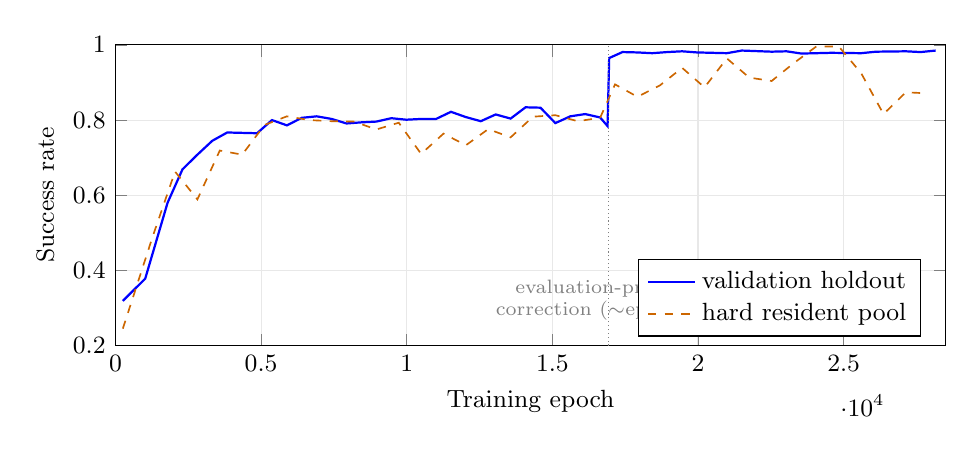
\begin{tikzpicture}
\begin{axis}[
  width=\linewidth, height=5.4cm,
  xlabel={Training epoch}, ylabel={Success rate},
  xmin=0, xmax=28500, ymin=0.2, ymax=1.0,
  legend pos=south east, legend cell align=left, legend style={font=\small},
  tick label style={font=\small}, label style={font=\small},
  grid=both, grid style={gray!18},
]
\addplot[thick, blue] coordinates {
(255,0.319)(1023,0.378)(1791,0.580)(2303,0.669)(2815,0.708)(3327,0.745)
(3839,0.767)(4351,0.766)(4863,0.765)(5375,0.800)(5887,0.786)(6399,0.806)
(6911,0.810)(7423,0.803)(7935,0.791)(8447,0.794)(8959,0.796)(9471,0.805)
(9983,0.801)(10495,0.803)(11007,0.803)(11519,0.822)(12031,0.808)(12543,0.797)
(13055,0.815)(13567,0.804)(14079,0.834)(14591,0.833)(15103,0.792)(15615,0.810)
(16127,0.816)(16639,0.807)(16895,0.784)(16950,0.965)(17407,0.981)(17919,0.980)
(18431,0.978)(18943,0.981)(19455,0.983)(19967,0.980)(20991,0.978)(21503,0.985)
(22527,0.982)(23039,0.983)(23551,0.977)(24575,0.979)(25599,0.978)(26111,0.982)
(27135,0.983)(27647,0.981)(28159,0.985)
};
\addlegendentry{validation holdout}
\addplot[semithick, orange!80!black, dashed] coordinates {
(255,0.245)(1279,0.490)(2047,0.663)(2815,0.589)(3583,0.719)(4351,0.708)
(5119,0.787)(5887,0.810)(6655,0.800)(7423,0.797)(8191,0.796)(8959,0.775)
(9727,0.793)(10495,0.710)(11263,0.764)(12031,0.733)(12799,0.776)(13567,0.754)
(14335,0.809)(15103,0.813)(15871,0.797)(16639,0.806)(17151,0.895)(17919,0.862)
(18687,0.892)(19455,0.939)(20223,0.887)(20991,0.964)(21759,0.913)(22527,0.904)
(23295,0.952)(24063,0.996)(24831,0.996)(25599,0.925)(26367,0.816)(27135,0.874)
(27903,0.871)
};
\addlegendentry{hard resident pool}
\draw[gray, densely dotted] (axis cs:16920,0.2) -- (axis cs:16920,1.0);
\node[anchor=south, font=\scriptsize, gray, align=center]
  at (axis cs:16920,0.24) {evaluation-protocol\\correction ($\sim$ep.\ 16.9k)};
\end{axis}
\end{tikzpicture}
\caption{Scheduled success during full-scale training.}\label{fig:learning_curve}
\end{figure}

The 98.47\% result supports strong tracking of the selected held-out
clip/body pairs under the specified threshold. It does not establish
all-body success for those clips, unseen-body generalization, or an untouched
test-set score. The thresholded success rate is complemented by position,
rotation, and smoothness measures because a successful rollout can still
have visible local errors or jitter.

% Evidence: note/README.note.md, section 76, recorded 2026-09-07.
% Do not replace the monitoring epoch with last.ckpt's epoch.
The run record is available at
\href{https://wandb.ai/yugoamaryl/hhi-protomotions/runs/3mvgad6f}
{the full-scale W\&B run}. The current table uses the recorded snapshot,
not a newly executed evaluation.


\subsection{Historical single-seed reference grid}
Cases A--D use refined references and E--H use unrefined references.
Within-run variation must not be interpreted as uncertainty across training
runs. The main architecture conclusion uses repeated refined runs instead.
\begin{table}[t]
\centering
\small
\caption{Historical seed-0 development grid. Success uncertainty is variation across eight evaluations within each run. Other columns are their means. Refined and unrefined policies track different targets. The three-seed comparison is in Table~\ref{tab:architecture_seeds}.}\label{tab:ablation_results}
\begin{tabularx}{\linewidth}{@{}llYrrrr@{}}
\toprule
Case & Architecture / data & Success (\%) & gt err & gr err & Jerk & HJ\% \\
\midrule
A & temporal MLP, refined        & 97.5 $\pm$ 0.8 & 0.109 & 0.207 & 1{,}729 & 33.3 \\
B & attention, refined           & 97.5 $\pm$ 1.4 & 0.098 & 0.228 & 3{,}455 & 40.4 \\
C & slot/type, refined           & \textbf{98.1 $\pm$ 0.6} & 0.097 & 0.226 & \textbf{1{,}757} & 34.2 \\
D & slot/type + AdaLN, refined   & 97.1 $\pm$ 1.2 & \textbf{0.090} & 0.220 & 3{,}145 & 38.9 \\
E & slot/type, unrefined         & 97.9 $\pm$ 0.6 & 0.102 & 0.219 & 1{,}422 & 29.6 \\
F & temporal MLP, unrefined      & 96.2 $\pm$ 1.6 & 0.115 & 0.212 & 2{,}927 & 36.6 \\
G & attention, unrefined         & 97.8 $\pm$ 1.2 & 0.098 & 0.219 & 3{,}117 & 34.9 \\
H & slot/type + AdaLN, unrefined & 97.5 $\pm$ 0.9 & 0.091 & 0.207 & 2{,}956 & 34.0 \\
\bottomrule
\end{tabularx}
\end{table}
\subsection{Full-scale run record}
The full-scale MorphMimic run shares the architecture of case C exactly (same
encoder, transformer, and head widths;
\texttt{mlp\_wide\_stage2\_discover\_attention\_slot\_type.py} inherits
these constants unchanged from the 150-clip experiment file), so its
parameter count is also 51,238,582. Parameter counts for the four
architectures (Table~\ref{tab:architecture_seeds}) are computed analytically
from each run's resolved model configuration, because every linear layer is
instantiated with \texttt{nn.LazyLinear} and has no fixed count outside a
materialized model. The run used six A40 GPUs (\texttt{ddp}, 32-bit, 2,048
environments and an 8,192 minibatch per GPU) for roughly 28,170 epochs; the
logged rank-0 wall time is about 77\,h, on the order of 450 GPU-hours. An
early restart after a memory-related failure resumed from the last checkpoint
with the resident pool reduced from 256 to 128 clips per rank and the local
cache multiplier set to 1.0; because configurations are reloaded from the
pickle on resume, the frozen configuration still records the pre-restart pool
size of 256. The earlier failed launch was logged into the same run.

\subsection{Reference refinement distributions}
Figure~\ref{fig:refine_dist} shows per-motion distributions (box: quartiles;
whiskers: 5th--95th percentile) over the 19,200 development references.
Stance-foot speed drops across almost the whole distribution, while position
jerk rises across almost the whole distribution.


\begin{figure}[t]
\centering
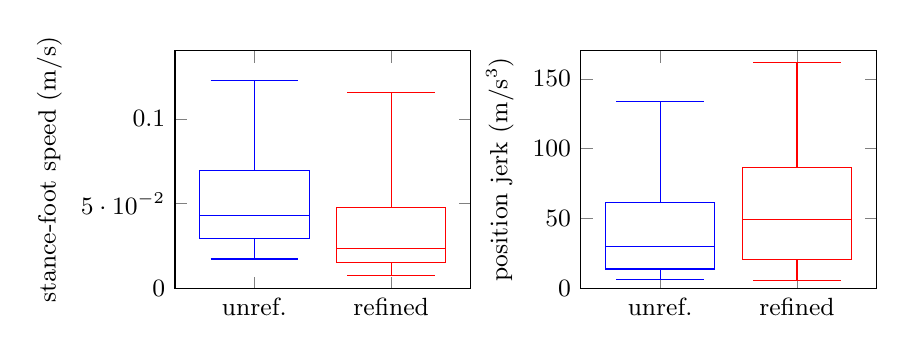
\begin{tikzpicture}
\begin{groupplot}[
  group style={group size=2 by 1, horizontal sep=1.4cm},
  width=0.44\linewidth, height=4.6cm,
  boxplot/draw direction=y, xtick={1,2}, xticklabels={unref., refined},
  tick label style={font=\small}, label style={font=\small},
]
\nextgroupplot[ylabel={stance-foot speed (m/s)}, ymin=0, ymax=0.14]
\addplot+[boxplot prepared={lower whisker=0.0174, lower quartile=0.0294,
  median=0.0430, upper quartile=0.0695, upper whisker=0.1228}] coordinates {};
\addplot+[boxplot prepared={lower whisker=0.0078, lower quartile=0.0151,
  median=0.0237, upper quartile=0.0476, upper whisker=0.1157}] coordinates {};
\nextgroupplot[ylabel={position jerk (m/s$^3$)}, ymin=0, ymax=170]
\addplot+[boxplot prepared={lower whisker=6.5, lower quartile=14.0,
  median=30.4, upper quartile=61.6, upper whisker=133.5}] coordinates {};
\addplot+[boxplot prepared={lower whisker=5.7, lower quartile=20.8,
  median=49.2, upper quartile=86.7, upper whisker=161.6}] coordinates {};
\end{groupplot}
\end{tikzpicture}
\caption{Reference sliding and jerk distributions before and after refinement.}\label{fig:refine_dist}
\end{figure}

\section{Additional Unseen-Body Results}\label{app:unseen_tables}
This appendix adds the coefficient-tier and mass-bin summary and the
checkpoint-regression list that support the unseen-body results. The complete
per-body results for both panels, 256 rows in total, are in Online Resource 1.

\subsection{Coefficient tiers and mass bins}
Table~\ref{tab:unseen_v2_groups} reports the predefined outside coefficient
tiers and descriptive simulated-mass bins on the 233-clip panel. Tier and mass
rows overlap, each partition covers all 128 bodies, and the mass thresholds are
the trained-asset range. These are associations, not identified causes.

\begin{table}[t]
\centering\small
\caption{Outside coefficient tiers and simulated-mass bins, 233-clip panel.}\label{tab:unseen_v2_groups}
\begin{tabular}{lrrr}
\toprule
Group & Bodies & Refined (\%) & Full-data (\%) \\
\midrule
$\|\beta\|_\infty\in(3,3.5]$ & 32 & 99.03 & 99.46 \\
$\|\beta\|_\infty\in(3.5,4]$ & 32 & 97.76 & 97.81 \\
$\|\beta\|_\infty\in(4,4.5]$ & 32 & 95.33 & 95.12 \\
$\|\beta\|_\infty\in(4.5,5]$ & 32 & 96.47 & 97.87 \\
\midrule
Mass $<26.4$ kg & 2 & 100.00 & 100.00 \\
Mass $26.4$--$144.4$ kg & 118 & 98.33 & 98.13 \\
Mass $>144.4$ kg & 8 & 79.02 & 88.62 \\
\bottomrule
\end{tabular}
\end{table}

\subsection{Checkpoint regressions}
Table~\ref{tab:unseen_v2_regressions} lists all bodies whose paired
success-change interval lies entirely below $-2$ percentage points on the
233-clip panel. These exploratory per-body intervals are not adjusted for
multiple comparisons.

\begin{table}[t]
\centering\small
\caption{Bodies with a paired success decrease beyond 2 percentage points.}\label{tab:unseen_v2_regressions}
\begin{tabular}{llrrr}
\toprule
Panel & Asset & Refined (\%) & Full-data (\%) & $\Delta$ (pp) \\
\midrule
Inside & \texttt{female\_e7bc8c92} & 92.3 & 79.0 & $-13.30$ \\
Inside & \texttt{male\_6d81a8f6} & 97.9 & 85.0 & $-12.88$ \\
Inside & \texttt{male\_ec3bb7f8} & 19.3 & 10.7 & $-8.58$ \\
Outside & \texttt{female\_edcf2449} & 94.8 & 58.4 & $-36.48$ \\
Outside & \texttt{male\_a7f6b877} & 65.7 & 40.8 & $-24.89$ \\
Outside & \texttt{male\_edcf2449} & 82.0 & 67.0 & $-15.02$ \\
Outside & \texttt{female\_e706da88} & 94.4 & 79.8 & $-14.59$ \\
Outside & \texttt{female\_bd0ec1ce} & 63.9 & 52.8 & $-11.16$ \\
Outside & \texttt{female\_f9bf3075} & 97.4 & 88.8 & $-8.58$ \\
\bottomrule
\end{tabular}
\end{table}


% Bibliography is kept in LaTeX to preserve the source-only update scope.
% Primary papers and official software repositories; checked during drafting.

\begin{thebibliography}{99}

\bibitem{amass}
Naureen Mahmood, Nima Ghorbani, Nikolaus F. Troje, Gerard Pons-Moll,
and Michael J. Black.
AMASS: Archive of Motion Capture as Surface Shapes.
In \emph{ICCV}, 2019.
\url{https://doi.org/10.1109/ICCV.2019.00554}.

\bibitem{humanml3d}
Chuan Guo, Shihao Zou, Xinxin Zuo, Sen Wang, Wei Ji, Xingyu Li,
and Li Cheng.
Generating Diverse and Natural 3D Human Motions From Text.
In \emph{CVPR}, 2022.
\url{https://doi.org/10.1109/CVPR52688.2022.00509}.

\bibitem{humos}
Shashank Tripathi, Omid Taheri, Christoph Lassner, Michael J. Black,
Daniel Holden, and Carsten Stoll.
HUMOS: Human Motion Model Conditioned on Body Shape.
In \emph{ECCV}, 2024.
\url{https://doi.org/10.1007/978-3-031-72640-8_8}.

\bibitem{deepmimic}
Xue Bin Peng, Pieter Abbeel, Sergey Levine, and Michiel van de Panne.
DeepMimic: Example-Guided Deep Reinforcement Learning of Physics-Based
Character Skills.
\emph{ACM Transactions on Graphics}, 37(4), 2018.
\url{https://doi.org/10.1145/3197517.3201311}.

\bibitem{phc}
Zhengyi Luo, Jinkun Cao, Alexander W. Winkler, Kris Kitani, and Weipeng Xu.
Perpetual Humanoid Control for Real-time Simulated Avatars.
In \emph{ICCV}, 2023.
\url{https://doi.org/10.1109/ICCV51070.2023.01000}.

\bibitem{ase}
Xue Bin Peng, Yunrong Guo, Lina Halper, Sergey Levine, and Sanja Fidler.
ASE: Large-Scale Reusable Adversarial Skill Embeddings for Physically
Simulated Characters. \emph{ACM Transactions on Graphics}, 41(4), Article 94, 2022.
\url{https://doi.org/10.1145/3528223.3530110}.

\bibitem{protomotions}
The ProtoMotions contributors.
ProtoMotions (official ProtoMotions 3 README, accessed 10 October 2026).
Open-source software for physics-based character animation and humanoid control.
\url{https://github.com/NVlabs/ProtoMotions}.

\bibitem{isaacgym}
Viktor Makoviychuk, Lukasz Wawrzyniak, Yunrong Guo, Michelle Lu, Kier Storey,
Miles Macklin, David Hoeller, Nikita Rudin, Arthur Allshire, Ankur Handa,
and Gavriel State.
Isaac Gym: High Performance GPU-Based Physics Simulation For Robot Learning.
Technical report, 2021.
\url{https://doi.org/10.48550/arXiv.2108.10470}.

\bibitem{ppo}
John Schulman, Filip Wolski, Prafulla Dhariwal, Alec Radford, and Oleg Klimov.
Proximal Policy Optimization Algorithms.
Technical report, 2017.
\url{https://doi.org/10.48550/arXiv.1707.06347}.

\bibitem{won2019}
Jungdam Won and Jehee Lee.
Learning Body Shape Variation in Physics-based Characters.
\emph{ACM Transactions on Graphics}, 38(6), Article 207, 2019.
\url{https://doi.org/10.1145/3355089.3356499}.

\bibitem{shapeverse}
Bharat Vyas and Carol O'Sullivan.
ShapeVerse: Physics-based Characters with Varied Body Shapes.
In \emph{Eurographics 2024 -- Posters}, 2024.
\url{https://doi.org/10.2312/egp.20241042}.

\bibitem{alborno2018}
Mazen Al Borno, Ludovic Righetti, Michael J. Black, Scott L. Delp,
Eugene Fiume, and Javier Romero.
Robust Physics-based Motion Retargeting with Realistic Body Shapes.
\emph{Computer Graphics Forum}, 37(8), 2018.
\url{https://doi.org/10.1111/cgf.13514}.

\bibitem{smpl}
Matthew Loper, Naureen Mahmood, Javier Romero, Gerard Pons-Moll,
and Michael J. Black.
SMPL: A Skinned Multi-Person Linear Model.
\emph{ACM Transactions on Graphics}, 34(6), 2015.
\url{https://doi.org/10.1145/2816795.2818013}.

\bibitem{smplsim}
Zhengyi Luo and contributors.
SMPLSim.
Open-source SMPL-family body-model simulation software.
\url{https://github.com/ZhengyiLuo/SMPLSim}.

\bibitem{attention}
Ashish Vaswani, Noam Shazeer, Niki Parmar, Jakob Uszkoreit, Llion Jones,
Aidan N. Gomez, Lukasz Kaiser, and Illia Polosukhin.
Attention Is All You Need.
In \emph{NeurIPS}, 2017.
\url{https://doi.org/10.48550/arXiv.1706.03762}.

\bibitem{dit}
William Peebles and Saining Xie.
Scalable Diffusion Models with Transformers.
In \emph{ICCV}, 2023.
\url{https://doi.org/10.1109/ICCV51070.2023.00387}.

\bibitem{pulse}
Zhengyi Luo, Jinkun Cao, Josh Merel, Alexander Winkler, Jing Huang,
Kris Kitani, and Weipeng Xu.
Universal Humanoid Motion Representations for Physics-Based Control.
In \emph{ICLR}, 2024.
\url{https://doi.org/10.48550/arXiv.2310.04582}.

\bibitem{omnih2o}
Tairan He, Zhengyi Luo, Xialin He, Wenli Xiao, Chong Zhang, Weinan Zhang,
Kris Kitani, Changliu Liu, and Guanya Shi.
OmniH2O: Universal and Dexterous Human-to-Humanoid Whole-Body
Teleoperation and Learning.
In \emph{CoRL}, 2024.
\url{https://doi.org/10.48550/arXiv.2406.08858}.

\bibitem{exbody2}
Mazeyu Ji, Xuanbin Peng, Fangchen Liu, Jialong Li, Ge Yang, Xuxin Cheng,
and Xiaolong Wang.
ExBody2: Advanced Expressive Humanoid Whole-Body Control.
Technical report, 2024.
\url{https://doi.org/10.48550/arXiv.2412.13196}.

\bibitem{gmt}
Zixuan Chen, Mazeyu Ji, Xuxin Cheng, Xuanbin Peng, Xue Bin Peng,
and Xiaolong Wang.
GMT: General Motion Tracking for Humanoid Whole-Body Control.
Technical report, 2025.
\url{https://doi.org/10.48550/arXiv.2506.14770}.

\bibitem{smp2020}
Wenlong Huang, Igor Mordatch, and Deepak Pathak.
One Policy to Control Them All: Shared Modular Policies for
Agent-Agnostic Control.
In \emph{ICML}, 2020.
\url{https://doi.org/10.48550/arXiv.2007.04976}.

\bibitem{wilson1927}
Edwin B. Wilson.
Probable Inference, the Law of Succession, and Statistical Inference.
\emph{Journal of the American Statistical Association}, 22(158), 209--212, 1927.
\url{https://doi.org/10.1080/01621459.1927.10502953}.

\end{thebibliography}

\end{document}
